\documentclass[11pt]{article}
\usepackage{amsmath,amssymb,amsthm,tikz}
\usepackage{url}
\usetikzlibrary{trees}

\newtheorem{definition}{Definition}
\newtheorem{theorem}{Theorem}
\newtheorem{claim}{Claim}

\newcommand{\eps}{\varepsilon}
\global\long\def\pp#1{\left(#1\right)}
\global\long\def\ppp#1{\left[#1\right]}




\newcommand{\handout}[5]{
  \noindent
  \begin{center}
  \framebox{
    \vbox{
      \hbox to 5.78in { {\bf CS 229r: Algorithms for Big Data } \hfill #2 }
      \vspace{4mm}
      \hbox to 5.78in { {\Large \hfill #5  \hfill} }
      \vspace{2mm}
      \hbox to 5.78in { {\em #3 \hfill #4} }
    }
  }
  \end{center}
  \vspace*{4mm}
}

\newcommand{\lecture}[4]{\handout{#1}{#2}{#3}{Scribe: #4}{Lecture #1}}
\newcommand{\bs}[1]{\boldsymbol{#1}}

% 1-inch margins, from fullpage.sty by H.Partl, Version 2, Dec. 15, 1988.
\topmargin 0pt
\advance \topmargin by -\headheight
\advance \topmargin by -\headsep
\textheight 8.9in
\oddsidemargin 0pt
\evensidemargin \oddsidemargin
\marginparwidth 0.5in
\textwidth 6.5in

\parindent 0in
\parskip 1.5ex


\begin{document}

\lecture{4 --- September 15, 2015}{Fall 2015}{Prof.\ Jelani Nelson}{Hyunghoon Cho}

\section{Recap}

Recall the following definition of {\it $p$-stable distributions.}
\begin{definition}
$D_{p}$ is a $p$-stable distribution on $\mathbf{R}$ if, for any $n$ independent samples $z_1,\dots,z_n$ from $D_p$, the following holds: $\forall x\in \mathbf{R}^n,  \sum_{i=1}^n x_iz_i \sim ||x||_p D_p$.
\end{definition}
In other words, any linear combination of a set of samples from a $p$-stable distribution must itself be a sample from the same distribution, scaled by the $p$-norm of the weight vector.
\begin{theorem}
A $p$-stable distribution exists iff $0<p\le 2$.
\end{theorem}
We know that the standard Gaussian distribution is 2-stable and the standard Cauchy distribution is 1-stable. Although in most cases a simple closed-form expression for $p$-stable distributions is not known, there is an efficient way to generate samples for any $p\in(0,2]$. If we let $\theta\in[-\frac{\pi}{2},\frac{\pi}{2}]$ and $r\in[0,1]$ be uniformly random samples, then
$$\frac{\sin(p\theta)}{\cos^{1/p}(\theta)}\pp{\frac{\cos(\theta(1-p))}{\ln(1/r)}}^{\frac{1-p}{p}}$$ 
is a sample from a $p$-stable distribution \cite{CMS76}.

\section{Indyk's Algorithm}

\subsection{Overview}

Let $\Pi=\{\pi_{ij}\}$ be an $m\times n$ matrix where every element $\pi_{ij}$ is sampled from a $p$-stable distribution, $D_p$. Given $x\in \mathbf{R}^n$, Indyk's algorithm \cite{Indyk06} estimates the $p$-norm of $x$ as 
$$ ||x||_p  \approx \text{median}_{i=1,\dots,m} |y_i|,$$
where $y=\Pi x$. Recall from last lecture that in a turnstile streaming model, each element in the stream reflects an update to an entry in $x$. While a naive algorithm would maintain $x$ in memory and calculate $||x||_p$ at the end, thus requiring $\Theta(n)$ space, Indyk's algorithm stores $y$ and $\Pi$. Combined with a space-efficient way to produce $\Pi$ (described later in the lecture) we achieve better space complexity.

\subsection{Analysis}
For simplicity of analysis, we will assume $\Pi$ is generated with $D_p$ such that if $Z\sim D_p$ then $\text{median}(|Z|) = 1$. In other words, we assume the probability mass of $D_p$ assigned to interval $[-1,1]$ is $1/2$. In addition, let $I_{[a,b]}(x)$ be an indicator function defined as
$$I_{[a,b]}(x)=\begin{cases}
1 & x\in[a,b],\\
0 & \text{otherwise}.
\end{cases}$$

Let $Z_i$ be the $i$-th row of $\Pi$. We have 
\begin{equation} \label{eq:yi}
y_i = \sum_{j=1}^n Z_{ij} x_j \sim ||x||_p D_p,
\end{equation}
which follows from the definition of $p$-stable distributions and noting that $Z_{ij}$'s are sampled from $D_p$. This implies 
\begin{equation} 
\mathbf{E} \ppp{ I_{[-1,1]} \pp{\frac{y_i}{||x||_p}} } = \frac{1}{2},
\end{equation}
since $y_i / ||x||_p \sim D_p$.

Moreover, it can be shown that
\begin{align}
\mathbf{E} \ppp{I_{[-1-\eps,1+\eps]}\pp{\frac{y_{i}}{||x||_{p}}}} &= \frac{1}{2}+\Theta(\eps), \\
\mathbf{E} \ppp{I_{[-1+\eps,1-\eps]}\pp{\frac{y_{i}}{||x||_{p}}}} &= \frac{1}{2}-\Theta(\eps).
\end{align}

Next, consider the following quantities:
\begin{align}
C_1 &= \frac{1}{m} \sum_i^m I_{[-1-\eps,1+\eps]}\pp{\frac{y_{i}}{||x||_{p}}}, \\
C_2 &= \frac{1}{m} \sum_i^m I_{[-1+\eps,1-\eps]}\pp{\frac{y_{i}}{||x||_{p}}}.
\end{align}

$C_1$ represents the fraction of $y_i$'s that satisfy $|y_i|\le (1+\eps) ||x||_p$, and similarly, $C_2$ represents the fraction of $y_i$'s that satisfy $|y_i|\le (1-\eps) ||x||_p$. By linearity of expectation, we have $\mathbf{E} [C_1] = 1/2 + \Theta(\eps)$ and $\mathbf{E} [C_2] = 1/2 - \Theta(\eps)$. Therefore, in expectation, the median of $|y_i|$ lies in $$[(1-\eps)||x||_p, (1+\eps)||x||_p]$$ as desired.

Now we analyze the variance of $C_1$ and $C_2$. We have
\begin{equation}
\mathbf{Var}\pp{C_1}=\frac{1}{m^{2}}\times m\times\text{(variance of the indicator variable)}.
\end{equation}
Since variance of any indicator variable is at most $1$, $\mathbf{Var} (C_1)\le \frac{1}{m}$. Similarly, $\mathbf{Var}(C_2)\le \frac{1}{m}$. With an appropriate choice of $m$ now we can ensure that the median of $|y_i|$ is in the desired $\eps$-range of $||x||_p$ with high probability.

\subsection{Derandomizing $\Pi$}

We have shown that Indyk's algorithm work, but independently generating and storing all $mn$ elements of $\Pi$ is expensive. Can we get by with a smaller degree of randomness? To invoke the definition of $p$-stable distributions for Equation \ref{eq:yi}, we need the entries in each row to be independent from one another. And the rows need to be pairwise independent for our calculation of variance to hold. As a side note, generating pairwise independent Gaussian or Cauchy random variables can be achieved by discretizing the space and treating them as discrete random variables. One can make a claim that, with fine enough discretization, the algorithm still succeeds with high probability.

Now suppose $w_{i}=\sum_{j=1}^n Q_{ij}x_{j}$ where $Q_{ij}$'s are $k$-wise independent $p$-stable distribution samples. What we want is an argument of the form 
\begin{equation}
\mathbf{E} \ppp{I_{[a,b]}\pp{\frac{w_{i}}{||x||_{p}}}} \approx_{\eps} \mathbf{E} \ppp{I_{[a,b]}\pp{\frac{y_{i}}{||x||_{p}}}}.
\end{equation}
If we can make such claim, then we can use $k$-wise independent samples in each row in lieu of fully independent samples to invoke the same arguments in the analysis above. This has been shown for $k=\Omega(1/\eps^{p})$ \cite{KNW10}, but we are not going to cover this in class. With this technique, we can specify $\Pi$ using only $O(k\lg n)$ bits; across rows, we only need to use 2-wise independent hash function that maps a row index to a $O(k\lg n)$ bit seed for the $k$-wise independent hash function. Indyk's approach to derandomizing $\Pi$, while the results are not as strong, employs a useful technique, so we will cover that here instead.

\subsubsection{Branching Programs}

A {\em branching program} can be described with a grid of nodes representing different states of the program---we can think of it as a DFA. The program starts at an initial node which is not part of the grid. At each step, the program reads $S$ bits of input, reflecting the fact that space is bounded by $S$, and makes a decision about which node in the subsequent column of the grid to jump to. After $R$ steps (number of columns in the grid), the final node visited by the program represents the outcome. The entire input, which can be represented as a length-$RS$ bit string, induces a distribution over the final states. Our goal is to generate the input string using fewer ($\ll RS$) random bits such that the original distribution over final states is well preserved. The following theorem addresses this goal.

\begin{theorem} (\cite{Nisan92}) \label{thm:nisan}
There exists $h:\{0,1\}^{t}\rightarrow\{0,1\}^{RS}$ for $t=O(S\lg R)$ such that 
\begin{equation}
\left| P_{x\sim U(\{0,1\}^{RS})}\left\{ f(B(x))=1 \right\} -P_{y\sim U(\{0,1\}^{t})}\left\{ f(B(h(y)))=1 \right\} \right| \le \frac{1}{2^{S}}.
\end{equation}
for any branching program $B$ and any function $f:\{0,1\}^{S}\rightarrow\{0,1\}$. 
\end{theorem}

In other words, such function $h$ can simulate the input to the branching program with only $t$ random bits such that it is almost impossible to discriminate the outcome of the simulated program from that of the original program.

\subsubsection{Nisan's Pseudorandom Generator (PRG)}

What does such a function look like? We start by taking a random sample $x$ from $\{0,1\}^S$. Then we place $x$ at the root and repeat the following procedure to create a complete binary tree. At each node, create two children and copy the string over to the left child. For the right child, use a random 2-wise independent hash function $h_j:[2^S]\rightarrow[2^S]$ chosen for the corresponding level of the tree and record the result of the hash. Once we reach $R$ levels, output the concatenation of all leaves, which is a length-$RS$ bit string. To illustrate, the first few levels of our tree would look like:

\begin{center}
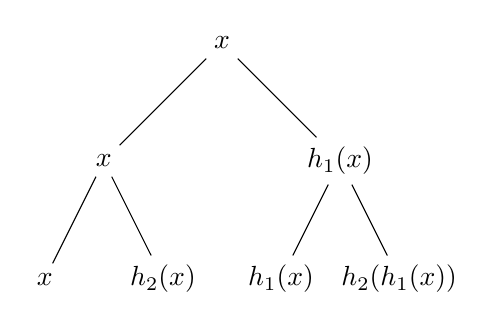
\begin{tikzpicture}[level distance=1.5cm,
  level 1/.style={sibling distance=3cm},
  level 2/.style={sibling distance=1.5cm}]
  \node {$x$}
    child {node {$x$}
      child {node {$x$}}
      child {node {$h_2(x)$}}
    }
    child {node {$h_1(x)$}
    child {node {$h_1(x)$}}
      child {node {$h_2(h_1(x))$}}
    };
\end{tikzpicture}
\end{center}

Since each hash function requires $S$ random bits and there are $\lg R$ levels in the tree, this function uses $O(S\lg R)$ bits total. We will not discuss why this function satisfies the condition in Theorem~\ref{thm:nisan}.

\subsubsection{Back to Indyk's Algorithm}
Now we will use Nisan's PRG to derandomize $\Pi$ in Indyk's algorithm. Consider the following program:

\begin{enumerate}
\item Initialize $c_1 \leftarrow 0$, $c_2 \leftarrow 0$
\item For $i=1,\dots,m$:
\begin{enumerate}
\item Initialize $y \leftarrow 0$
\item For $j=1,\dots,n$:
\begin{enumerate}
\item Update $y \leftarrow y + \pi_{ij} x_j $
\end{enumerate}
\item If $y \le (1+\eps) ||x||_p$, then increment $c_1$
\item If $y \le (1-\eps) ||x||_p$, then increment $c_2$
\end{enumerate}

\end{enumerate}

Note that this program only uses $O(\lg n)$ bits and is a branching program that mimics the proof of correctness for Indyk's algorithm. More specifically, Indyk's algorithm succeeded iff at the end of this program $c_1 > \frac{m}{2}$ and $c_2 < \frac{m}{2}$. The only source of randomness in this program are the $\pi_{ij}$'s. We will use Nisan's PRG to produce these random numbers. We invoke Theorem \ref{thm:nisan} with the above program as $B$ and an indicator function checking whether the algorithm succeeded or not as $f$. Note that the space bound is $S=O(\lg n)$ and the number of steps taken by the program is $R=O(mn)$, or $O(n^2)$ since $m\le n$. This means we can ``fool'' the proof of correctness of Indyk's algorithm only using $O(\lg^2 n)$ random bits to generate $\Pi$. 

\section{The $p>2$ Case}

Indyk's algorithm uses $p$-stable distributions which only exist for $p\in (0,2]$. What do we do when $p>2$?

\begin{theorem}
$n^{1-2/p}\text{poly}(\frac{\lg n}{\eps})$ space is necessary and
sufficient.
\end{theorem}

A nearly optimal lower bound was given by \cite{BarYossef04} and first achieved by \cite{IW05}. In this lecture we will discuss the algorithm of \cite{Andoni12}, which is based on \cite{AKO11} and \cite{JST11}. We will focus on $\eps = \Theta(1)$. Refining this result may be included in the next homework.

In this algorithm, we let $\Pi=PD$. $P$ is a $m\times n$ matrix, where each column has a single non-zero element that is either $1$ or $-1$. $D$ is a $n\times n$ diagonal matrix with $d_{ii}=u_{i}^{-1/p}$, where $u_{i}\sim \text{Exp}(1)$. In other words, $$P\{u_{i}>t\}=\begin{cases}
1 & t\le0,\\
e^{-t} & t>0.
\end{cases}$$

Similar to the $0<p\le 2$ case, we will keep $y=\Pi x$, but here we estimate $||x||_p$ with
\begin{equation}
||x||_p \approx ||y||_{\infty}=\max_{i}|y_{i}|.
\end{equation}

\begin{theorem} \label{thm:andoni}
$P\left\{\frac{1}{4}||x||_{p}\le||y||_{\infty}\le4||x||_{p}\right\}\ge\frac{11}{20}$ for $m=\Theta(n^{1-2/p}\lg n)$.
\end{theorem}

Let $z=Dx$, which means $y=Pz$. To prove Theorem \ref{thm:andoni}, we will first show that $||z||_\infty$ provides a good estimate and then show that applying $P$ to $z$ preserves this. The latter step is deferred to next class due to time constraints.

\begin{claim}
$P\left\{ \frac{1}{2}||x||_{p}\le||z||_{\infty}\le2||x||_{p} \right\}\ge\frac{3}{4}$
\end{claim}
\begin{proof}
Let $q=\min\left\{\frac{u_{1}}{|x_{1}|^{p}},\dots,\frac{u_{n}}{|x_{n}|^{p}}\right\}$. We have 
\begin{align}
P\{q>t\} & = P\left\{ \forall i,u_{i}>t|x_{i}|^{p} \right\}\\
 & = \prod_{i=1}^ne^{-t|x_{i}|^{p}}\\
 & = e^{-t||x||_{p}^{p}},
\end{align}
which implies $q\sim \frac{Exp(1)}{|x||_{p}^{p}}$. Thus,
\begin{align}
P\left\{\frac{1}{2}||x||_{p}\le||z||_{\infty}\le2||x||_{p}\right\} &= P\left\{\frac{1}{2^{p}}||x||_{p}^{-p}\le q\le2^{p}||x||_{p}^{-p}\right\} \\
&=e^{-\frac{1}{2^{p}}}-e^{-2^{p}} \\
&\ge\frac{3}{4},
\end{align}
for $p>2$.

\end{proof}

\bibliographystyle{alpha}

\begin{thebibliography}{42}

\bibitem[CMS76]{CMS76}
J. M.~Chambers, C. L.~Mallows, and B. W.~Stuck.
\newblock A method for simulating stable random variables.
\newblock {\em Journal of the american statistical association}, 71.354 (1976): 340-344.

\bibitem[KNW10]{KNW10}
Daniel~Kane, Jelani~Nelson, David~Woodruff.
\newblock On the exact space complexity of sketching and streaming small norms.
\newblock {\em Proceedings of the twenty-first annual ACM-SIAM symposium on Discrete Algorithms (SODA)}, 2010.

\bibitem[BarYossef04]{BarYossef04}
Ziv~Bar-Yossef, T. S.~Jayram, Ravi~Kumar, and D.~Sivakumar
\newblock An information statistics approach to data stream and communication complexity.
\newblock {\em Journal of Computer and System Sciences}, 68 (2004): 702-732.

\bibitem[Andoni12]{Andoni12}
Alexandr~Andoni.
\newblock High frequency moments via max-stability. 
\newblock Manuscript, 2012. \url{http://web.mit.edu/andoni/www/papers/fkStable.pdf}

\bibitem[AKO11]{AKO11}
Alexandr~Andoni, Robert~Krauthgamer, Krzysztof~Onak.
\newblock Streaming Algorithms via Precision Sampling.
\newblock {\em FOCS}, pgs.\ 363--372, 2011.

\bibitem[JST11]{JST11}
Hossein~Jowhari, Mert~Saglam, G\'{a}bor~Tardos.
\newblock Tight bounds for $L_p$ samplers, finding duplicates in streams, and related problems.
\newblock {\em PODS}, pgs.\ 49--58, 2011.

\bibitem[Indyk06]{Indyk06}
Piotr~Indyk.
\newblock Stable distributions, pseudorandom generators, embeddings, and data stream computation.
\newblock {\em J. ACM} 53(3): 307--323, 2006.

\bibitem[IW05]{IW05}
Piotr~Indyk, David~P.~Woodruff.
\newblock Optimal approximations of the frequency moments of data streams. 
\newblock {\em STOC}, pgs.\ 202--208, 2005.

\bibitem[Nisan92]{Nisan92}
Noam~Nisan.
\newblock Pseudorandom Generators for Space-Bounded Computation.
\newblock {\em Combinatorica}, 12(4):449-461, 1992.

\end{thebibliography}


\end{document}